\documentclass[a4paper]{article}
\usepackage[utf8]{inputenc}
\usepackage[spanish, es-tabla, es-noshorthands]{babel}
\usepackage[table,xcdraw]{xcolor}
\usepackage[a4paper, footnotesep = 1cm, width=20cm, top=2.5cm, height=25cm, textwidth=18cm, textheight=25cm]{geometry}
%\geometry{showframe}

\usepackage{tikz}
\usepackage{amsmath}
\usepackage{amsfonts}
\usepackage{amssymb}
\usepackage{float}
\usepackage{graphicx}
\usepackage{caption}
\usepackage{subcaption}
\usepackage{multicol}
\usepackage{multirow}
\setlength{\doublerulesep}{\arrayrulewidth}
\usepackage{booktabs}

\usepackage{hyperref}
\hypersetup{
    colorlinks=true,
    linkcolor=blue,
    filecolor=magenta,      
    urlcolor=blue,
    citecolor=blue,    
}

\newcommand{\quotes}[1]{``#1''}
\usepackage{array}
\newcolumntype{C}[1]{>{\centering\let\newline\\\arraybackslash\hspace{0pt}}m{#1}}
\usepackage[american]{circuitikz}
\usetikzlibrary{calc}
\usepackage{fancyhdr}
\usepackage{units} 

\graphicspath{{../Ejercicio-1/}{../Ejercicio-2/}{../Ejercicio-3/}{../Ejercicio-4/}}

\pagestyle{fancy}
\fancyhf{}
\lhead{22.01 Teoría de Circuitos}
\rhead{Mechoulam, Lambertucci, Rodriguez Turco, Londero, Galdeman}
\rfoot{\centering \thepage}

\begin{document}

%%%%%%%%%%%%%%%%%%%%%%%%%
%		Caratula		%
%%%%%%%%%%%%%%%%%%%%%%%%%

\begin{titlepage}
\newcommand{\HRule}{\rule{\linewidth}{0.5mm}}
\center
\mbox{\textsc{\LARGE \bfseries {Instituto Tecnológico de Buenos Aires}}}\\[1.5cm]
\textsc{\Large 22.01 Teoría de Circuitos}\\[0.5cm]


\HRule \\[0.6cm]
{ \Huge \bfseries Trabajo práctico N$^{\circ}$5}\\[0.4cm] 
\HRule \\[1.5cm]


{\large

\emph{Grupo 3}\\
\vspace{3px}

\begin{tabular}{lr} 	
\textsc{Mechoulam}, Alan  &  58438\\
\textsc{Lambertucci}, Guido Enrique  & 58009 \\
\textsc{Rodriguez Turco}, Martín Sebastian  & 56629 \\
\textsc{Londero Bonaparte}, Tomás Guillermo  & 58150 \\
\textsc{Galdeman}, Agustín & 59827\\
\end{tabular}

\vspace{20px}

\emph{Profesores}\\
Jacoby, Daniel Andrés\\
Belaustegui Goitia, Carlos\\
Iribarren, Rodrigo Iñaki\\
\vspace{3px}
%\textsc{} \\	

\vspace{100px}

\begin{tabular}{ll}

Presentado: & */*/19\\

\end{tabular}

}

\vfill

\end{titlepage}


%%%%%%%%%%%%%%%%%%%%%
%		Indice		%
%%%%%%%%%%%%%%%%%%%%%

\tableofcontents
\newpage

%%%%%%%%%%%%%%%%%%%%%
%		Informe		%
%%%%%%%%%%%%%%%%%%%%%

\section{Introducción}
En este informe se presenta y se explica como se confeccionó el filtro final propuesto por la cátedra. Para este, se valió del uso de las aproximaciones y celdas estudiadas a lo largo de la materia, para luego poder satisfacer la plantilla establecida.

\section{Elaboración del filtro}
Dado que el filtro debe ser un rechaza banda, con aproximación de Chebycheff Inverso, se buscó que este cumpla con las siguientes restricciones:
\begin{table}[H]
\centering
\begin{tabular}{cc}
\hline
\textbf{Variable} & \textbf{Valor} \\
\hline
$f_p^-$ & 11.712 kHz   \\ 
$f_a^-$ & 13.802kHz    \\ 
$f_a^+$ & 16.301kHz    \\ 
$f_p^+$ & 19.211kHz    \\ 
$A_a$   & 45dB         \\ 
$A_p$   & 1dB          \\ 
k       & $\frac{1}{3}$ \\ 
\hline
\end{tabular}
\caption{Características del filtro realizado.}
\label{tabla:caracteristicas1}
\end{table}

Para ello, se decidió emplear celdas del tipo universal, más específicamente una Fleischer-Tow. Es por ello que se analiza y se explica la selección de dicho tipo de celda a continuación. 

\subsection{Celda universal Fleischer-Tow (FT)}
En ocasiones es deseable poseer una señal de entrada que alimente varios nodos, obteniendo una única salida. A continuación se presenta la celda Fleischer-Tow, la cual se caracteriza por poder presentar una única transferencia que, dependiendo de los componentes seleccionados, puede ser un pasa bajos, pasa altos, pasa todo, de banda pasante y rechaza banda\footnote{R. Raut and M. N. S. Swamy, Modern Analog Filter Analysis and Design, 1st. ed. Weinheim: John Wiley and Sons, 2010.}, lo cual es una fuerte ventaja frente a los otros tipos de celdas universales, las cuales requieren más de tres operacionales para conseguir dichas salidas.

\begin{figure}[H]
\centering
	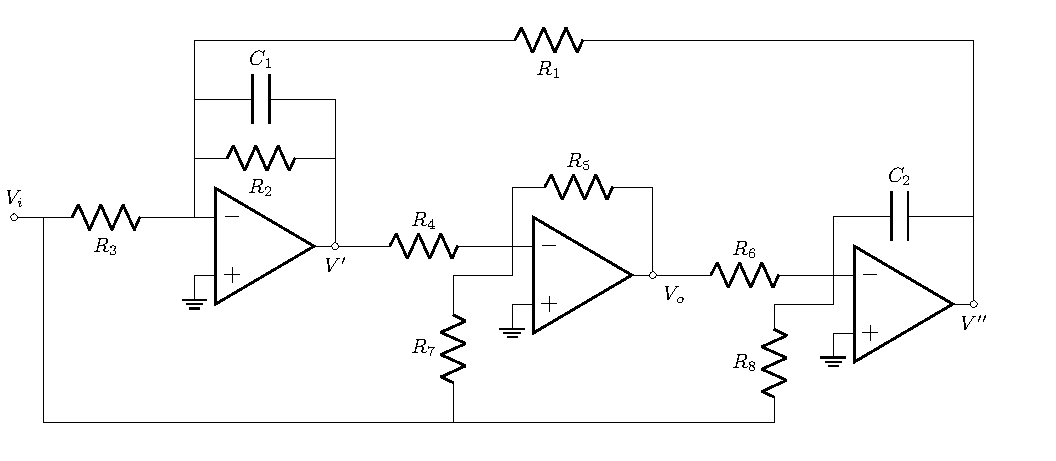
\includegraphics[width=0.9\textwidth]{Imagenes/FT.pdf}
	\caption{Circuito de la celda Universal Fleischer-Tow.}
\label{fig:FT}
\end{figure}

Se analiza el circuito presentado para poder obtener la transferencia de este. Para calcular la función mencionada de esta celda, se observa primero la siguiente configuración:
\begin{figure}[H]
\centering
\begin{circuitikz}
	\node [ocirc, label=left:$V_a$](va){};
	\draw (va.east) to[generic, l=$Z_1$] ++(3,0) node[op amp, anchor=-](A1){};
	\draw (va) ++(0.5,0) node[](v1aux1){};
	\draw (A1.+) node[ground](){};
	\draw (A1.out) node[](aux1){};	
	\draw (A1.-) -- ++(0,1) to[generic, l=$Z_3$] ++(2.25,0) -| (aux1.center);
	\draw (A1.out) -- ++(0.5,0) node[ocirc, label=below:$V_c$](){};
	\draw (A1.-) -- ($ (A1.-) !.7! (A1.+) $) to[generic, l=$Z_2$] ++(-3,0) node[ocirc, label=left:$V_b$](vb){};
\end{circuitikz}
\caption{Circuito genérico inversor.}
\label{fig:generic}
\end{figure}

Observando la Figura (\ref{fig:generic}), aplicando el teorema de superposición, se presenta una configuración inversora, por lo que se obtiene
\begin{equation}
	V_c = -\frac{V_a}{\frac{Z_1}{Z_3} + \frac{Z_1}{Z_3 A_o} + \frac{1}{A_o}} - \frac{V_b}{\frac{Z_2}{Z_3} + \frac{Z_2}{Z_3 A_o} + \frac{1}{A_o}}
	\label{equ:generic}
\end{equation}

Aplicando (\ref{equ:generic}) y considerando los tres operacionales de la Figura (\ref{fig:FT}) iguales, se obtiene el siguiente sistema de ecuaciones:
\begin{equation}
\begin{split}
	V' = - V_i A - V'' B \\
	V_o = - V' C - V_i D \\
	V'' = - V_o E - V_i F
\end{split}
\end{equation}
siendo las constantes empleadas las siguientes:
\begin{equation}
\begin{split}
	A^{-1} =& \ \frac{R_3}{R_2 // \frac{1}{sC_1}} + \frac{R_3}{\left( R_2 // \frac{1}{sC_1} \right) A_o} + \frac{1}{A_o} \\
	B^{-1} =& \ \frac{R_1}{R_2 // \frac{1}{sC_1}} + \frac{R_1}{\left( R_2 // \frac{1}{sC_1} \right) A_o} + \frac{1}{A_o} \\
	C^{-1} =& \ \frac{R_4}{R_5} + \frac{R_4}{R_5 A_o} + \frac{1}{A_o} \\
	D^{-1} =& \ \frac{R_7}{R_5} + \frac{R_7}{R_5 A_o} + \frac{1}{A_o} \\
	E^{-1} =& \ sC_2R_6 + \frac{sC_2R_6}{A_o} + \frac{1}{A_o} \\
	F^{-1} =& \ sC_2R_8 + \frac{sC_2R_8}{A_o} + \frac{1}{A_o}
\end{split}
\end{equation}

Operando algebraicamente, se obtiene que la transferencia de esta configuración es
\begin{equation}
	\frac{V_o}{V_i} = \frac{AC - BCF - D}{1 + BCE}
	\label{equ:transf-ft-r}
\end{equation}

Si se consideran ideales los operacionales, es decir, se toma $A_o \rightarrow \infty$, se obtiene que la forma de la transferencia final es
\begin{equation}
	\frac{V_o}{V_i} = - \frac{R_6}{R_8} \frac{s^{2} \frac{C_1 C_2 R_1 R_8 R_4}{R_7} + s \frac{C_2 R_1 R_8 R_4}{R_2} \left( \frac{1}{R_7} - \frac{R_2}{R_3 R_4} \right) + 1}{s^{2} \frac{C_1 C_2 R_6 R_1 R_4}{R_5} + s \frac{C_2 R_6 R_1 R_4}{R_2 R_5} + 1}
\label{equ:transf-ft-i}
\end{equation}

Es de interés obtener de esta los factores $\omega_o$ y $Q$ de los polos, siendo estos los presentados a continuación.
\begin{equation}
\begin{split}
	\omega_o = \sqrt{\frac{R_5}{R_6 R_1 R_4 C_1 C_2}} \\
	Q = R_2 \sqrt{\frac{C_1 R_5}{C_2 R_6 R_1 R_4}} 
\end{split}
\label{equ:woq-ft}
\end{equation}

Es así que se destaca la dependencia de $\omega_o$ y $Q$ de los capacitores, mientras que resultan ser independientes de $R_8$. Además, se destaca la que la frecuencia del polo es independiente de la resistencia $R_2$, mientras que $Q$ no, lo que permite modificar la primer variable sin afectar a la segunda.

\subsection{Análisis de sensibilidades}
En la siguiente sección, se procede a calcular las sensibilidades de $H(s)$, $Q$ y $\omega_o$ con respecto de cada componente, definiéndose la sensibilidad de una función $y$ con respecto de $x$ de la forma:
\begin{equation*}
	S_{x}^{y} = \frac{\delta y}{\delta x} \frac{x}{y}
\end{equation*}

Primero, se presentan las sensibilidades de $H\left(s \right)$:
\begin{equation}
S_{R_2}^{H} = -{\frac {s \left[ s{C_2}\,{R_6}\,{R_1}\,{R_8}\,{R_7}+{
R_3}\, \left( -{R_6}\,{R_7}+{R_8}\,{R_5} \right) 
 \right] {C_2}\,{R_2}\,{R_1}\,{R_4}}{ \left[ {R_2}\,{
R_5}+{R_1}\, \left( {C_1}\,{R_2}\,s+1 \right) {R_4}\,s{
C_2}\,{R_6} \right]  \left[ s{R_1}\,{R_8}\, \left( {C_1
}\,{R_2}\,{R_3}\,{R_4}\,s-{R_2}\,{R_7}+{R_3}\,{R_4} \right) {C_2}+{R_2}\,{R_3}\,{R_7} \right] }}
\end{equation}

\begin{equation}
S_{R_6}^{H} =	{\frac {{R_2}\,{R_5}}{{R_1}\, \left( {C_1}\,{R_2}\,s+1
 \right) {R_4}\,s{C_2}\,{R_6}} \left[ {\frac {{R_2}\,{R_5}}{{R_1}\, \left( {C_1}\,{R_2}\,s+1 \right) {R_4}\,s{
C_2}\,{R_6}}}+1 \right] ^{-1}}
\end{equation}

\begin{equation}
S_{R_1}^{H} = {\frac { \left\lbrace  \left[ s{C_1}\,{R_3}\, \left( -{R_6}\,{R_7}+{R_8}\,{R_5} \right) {R_4}-{R_5}\,{R_8}\,{R_7}
 \right] {R_2}+{R_4}\,{R_3}\, \left( -{R_6}\,{R_7}+{
R_8}\,{R_5} \right)  \right\rbrace s{C_2}\,{R_2}\,{R_1}}{
 \left[  \left( {C_1}\,{C_2}\,{R_6}\,{R_1}\,{R_4}\,{s}^
{2}+{R_5} \right) {R_2}+{R_1}\,{R_4}\,s{C_2}\,{R_6}
 \right]  \left\lbrace  \left[ {s}^{2}{R_4}\,{C_1}\,{C_2}\,{R_1}
\,{R_3}\,{R_8}-{R_7}\, \left( {C_2}\,{R_1}\,{R_8}\,s
-{R_3} \right)  \right] {R_2}+{R_1}\,{R_4}\,s{C_2}\,{
R_8}\,{R_3} \right\rbrace }}
\end{equation}

\begin{equation}
S_{R_3}^{H} = -{\frac {{R_2}\,{R_5}}{{R_3}\, \left( {C_1}\,{R_2}\,s+1
 \right) {R_4}} \left[ -{\frac {{R_2}\,{R_5}}{{R_1}\,
 \left( {C_1}\,{R_2}\,s+1 \right) {R_4}\,s{C_2}\,{R_8}}
}+{\frac {{R_2}\,{R_5}}{{R_3}\, \left( {C_1}\,{R_2}\,s+
1 \right) {R_4}}}-{\frac {{R_5}}{{R_7}}} \right] ^{-1}}
\end{equation}

\begin{equation}
s_{R_8}^{H} ={\frac {{R_2}\,{R_5}}{{R_1}\, \left( {C_1}\,{R_2}\,s+1
 \right) {R_4}\,s{C_2}\,{R_8}} \left[ -{\frac {{R_2}\,{
R_5}}{{R_1}\, \left( {C_1}\,{R_2}\,s+1 \right) {R_4}\,s
{C_2}\,{R_8}}}+{\frac {{R_2}\,{R_5}}{{R_3}\, \left( {
C_1}\,{R_2}\,s+1 \right) {R_4}}}-{\frac {{R_5}}{{R_7}}}
 \right] ^{-1}}
\end{equation}

\begin{equation}
S_{R_7}^{H} ={\frac {{R_5}}{{R_7}} \left[ -{\frac {{R_2}\,{R_5}}{{R_1}\, \left( {C_1}\,{R_2}\,s+1 \right) {R_4}\,s{C_2}\,{
R_8}}}+{\frac {{R_2}\,{R_5}}{{R_3}\, \left( {C_1}\,{
R_2}\,s+1 \right) {R_4}}}-{\frac {{R_5}}{{R_7}}} \right]^{-1}}
\end{equation}

\begin{equation}
S_{R_4}^{H} = {\frac { s \left( {C_1}\,{R_2}\,s+1 \right) \left[ s{C_2}\,{
R_6}\,{R_1}\,{R_8}\,{R_7}+{R_3}\, \left( -{R_6}\,{
R_7}+{R_8}\,{R_5} \right)  \right] {C_2}\,{R_2}\,{R_1}\,{R_4}}{ \left( {C_1}\,{C_2}\,{R_2}\,{R_6}\,{R_1
}\,{R_4}\,{s}^{2}+{R_1}\,{R_4}\,s{C_2}\,{R_{6}}+{R_2}
\,{R_5} \right)  \left[ {s}^{2}{R_4}\,{C_1}\,{C_2}\,{R_2}\,{R_1}\,{R_3}\,{R_8}+{C_2}\,{R_1}\,{R_8}\,
 \left( -{R_2}\,{R_7}+{R_3}\,{R_4} \right) s+{R_2}\,{
R_3}\,{R_7} \right] }}
\end{equation}

\begin{equation}
S_{R_5}^{H} = {\frac {{R_1}\, \left( {C_1}\,{R_2}\,s+1 \right) {R_4}\,s{
C_2}\,{R_6}}{{R_2}\,{R_5}+{R_1}\, \left( {C_1}\,{
R_2}\,s+1 \right) {R_4}\,s{C_2}\,{R_6}}}
\end{equation}

\begin{equation}
S_{C_1}^{H} = {\frac {{C_1}\,{s}^{2} \left[ s{C_2}\,{R_6}\,{R_1}\,{R_8}\,{R_7}+{R_3}\, \left( -{R_6}\,{R_7}+{R_8}\,{R_5}
 \right)  \right] {C_2}\,{{R_2}}^{2}{R_1}\,{R_4}}{ \left[ 
{R_2}\,{R_5}+{R_1}\, \left( {C_1}\,{R_2}\,s+1 \right) {
R_4}\,s{C_2}\,{R_6} \right]  \left[ s{R_1}\,{R_8}\,
 \left( {C_1}\,{R_2}\,{R_3}\,{R_4}\,s-{R_2}\,{R_7}+{
R_3}\,{R_4} \right) {C_2}+{R_2}\,{R_3}\,{R_7}
 \right] }}
\end{equation}

\begin{equation}
S_{C_2}^{H} = {\frac { \left\lbrace  \left[ s{C_1}\,{R_3}\, \left( -{R_6}\,{R_7}+{R_8}\,{R_5} \right) {R_4}-{R_5}\,{R_8}\,{R_7}
 \right] {R_2}+{R_4}\,{R_3}\, \left( -{R_6}\,{R_7}+{
R_8}\,{R_5} \right)  \right\rbrace s{C_2}\,{R_2}\,{R_1}}{
 \left[  \left( {C_1}\,{C_2}\,{R_6}\,{R_1}\,{R_4}\,{s}^
{2}+{R_5} \right) {R_2}+{R_1}\,{R_4}\,s{C_2}\,{R_6}
 \right]  \left\lbrace  \left[ {s}^{2}{R_4}\,{C_1}\,{C_2}\,{R_1}
\,{R_3}\,{R_8}-{R_7}\, \left( {C_2}\,{R_1}\,{R_8}\,s
-{R_3} \right)  \right] {R_2}+{R_1}\,{R_4}\,s{C_2}\,{
R_8}\,{R_3} \right\rbrace }}
\end{equation}

Luego, dado que la sensibilidades de $\omega_o$ y $Q$ resultan constantes, independientemente del componente del cual se las calcula, se presenta dichos valores de interés en la siguiente tabla.
\begin{table}[H]
\centering
\begin{tabular}{ccccccccccc}
\hline
 & $\mathbf{R_2}$ & $\mathbf{R_6}$ & $\mathbf{R_1}$ & $\mathbf{R_3}$ & $\mathbf{R_8}$ & $\mathbf{R_7}$ & $\mathbf{R_4}$ & $\mathbf{R_5}$ & $\mathbf{C_1}$ & $\mathbf{C_2}$ \\
\hline
$\omega_o$ & 0 & -0.5 & -0.5 & 0 & 0 & 0 & -0.5 & 0.5 & -0.5 & -0.5 \\
$Q$ & 1 & -0.5 & -0.5 & 0 & 0 & 0 & -0.5 & 0.5 & 0.5 & -0.5	\\
\hline
\end{tabular}
\caption{Sensibilidades de $\omega_o$ y $Q$ con respecto de cada componente}
\end{table}

\section{Selección de componentes}
Elección de componentes:
\begin{table}[H]
\centering
\begin{tabular}{ccc}
\hline
\multicolumn{1}{c}{Componente} & \multicolumn{1}{c}{Valor} & Composición \\ \hline
$R_1$                           & 33.68K                     & 680+33K     \\
$R_2$                           & 334.28K                    & 3.9K+330K   \\
$R_3$                           & 47K                        & 47K         \\
$R_4$                           & 334.28K                    & 3.9K+330K   \\
$R_5$                           & 47K                        & 47K         \\
$R_6$                           & 49.7K                        & 2.7k+47k         \\
$R_7$                           & 47K                        & 47K         \\
$R_8$                           & 50K                        & 47K+3k         \\
$C_1$                           & 95P                        & 68p//27p     \\
$C_2$                           & 95P                        & 68p //27p    \\
\hline
\end{tabular}
\caption{Componentes seleccionados de la primer etapa.}
\end{table}

\begin{table}[H]
\centering
\begin{tabular}{ccc}
\hline
\multicolumn{1}{c}{Componente} & \multicolumn{1}{c}{Valor} & Composición  \\ \hline
$R_1$                           & 27.03                      & 27+27K      \\
$R_2$                           & 371.57k                    & 680k // 820k \\
$R_3$                           & 47k                        & 47k          \\
$R_4$                           & 371.57k                    & 680k //820k   \\
$R_5$                           & 52.5k                      & 56k//820k    \\
$R_6$                           & 49.77k                     & 2.7k+47k     \\
$R_7$                           & 47k                        & 47k          \\
$R_8$                           & 47.5k                        & 47k+500          \\
$C_1$                           & 100p                       & 100p         \\
$C_2$  \\
\hline
\end{tabular}
\caption{Componentes seleccionados de la segunda etapa.}
\end{table}

\begin{table}[H]
\centering
\begin{tabular}{ccc}
\hline
\multicolumn{1}{c}{Componente} & \multicolumn{1}{c}{Valor} & Composición \\ \hline
$R_1$                           & 27.13                      & 120+27k     \\
$R_2$                           & 465.31k                    & 680k//1.5M  \\
$R_3$                           & 47k                        & 47k         \\
$R_4$                           & 465.31k                    & 680k//1.5M  \\
$R_5$                           & 42.08k                     & 15k+27k     \\
$R_6$                           & 49.77k                     & 2.7k+47k    \\
$R_7$                           & 47k                        & 47k         \\
$R_8$                           & 48k                        & 47k+1k         \\
$C_1$                           & 100p                       & 100p        \\
$C_2$                           & 100p                       & 100p        \\
\hline
\end{tabular}
\caption{Componentes seleccionados de la tercer etapa.}
\end{table}

\begin{table}[H]
\centering
\begin{tabular}{ccc}
\hline
\multicolumn{1}{c}{Componente} & \multicolumn{1}{c}{Valor} & Composición \\ \hline
$R_1$                           & 10.29k                     & 4.7k+5.6k   \\
$R_2$                           & 1.32M                      & 120k+1.2M   \\
$R_3$                           & 47k                        & 47k         \\
$R_4$                           & 1.32M                      & 120k+1.2M   \\
$R_5$                           & 39.44k                     & 470+39k     \\
$R_6$                           & 49.77K                     & 2.7k+47k    \\
$R_7$                           & 47k                        & 47k         \\
$R_8$                           & 48k                        & 47k+1k         \\
$C_1$                           & 92p                        & 10p // 82p  \\
$C_2$                           & 92p                        & 10p // 82p  \\
\hline
\end{tabular}
\caption{Componentes seleccionados de la cuarta etapa.}
\end{table}

\begin{table}[H]
\centering
\begin{tabular}{ccc}
\hline
\multicolumn{1}{c}{Componente} & \multicolumn{1}{c}{Valor} & Composición \\ \hline
$R_1$                           & 10.19k                     & 12k//68k    \\
$R_2$                           & 918.2k                     & 100k+820k   \\
$R_3$                           & 47k                        & 47k         \\
$R_4$                           & 918.2k                     & 100k+820k   \\
$R_5$                           & 56k                        & 56k         \\
$R_6$                           & 49.77k                     & 2.7k+47k    \\
$R_7$                           & 45k                        & 43k+2k         \\
$R_8$                           & 55k                        & 12k+43k         \\
$C_1$                           & 88p                      & 82p//5.6p    \\
$C_2$                           & 88p                      & 82p//5.6p   \\
\hline
\end{tabular}
\caption{Componentes seleccionados de la quinta etapa.}
\end{table}

\begin{table}[H]
\centering
\begin{tabular}{ccc}
\hline
\multicolumn{1}{c}{Componente} & \multicolumn{1}{c}{Valor} & Composición \\ \hline
$R_1$                           & 27.13                      & 120+27k     \\
$R_2$                           & 465.31k                    & 680k//1.5M  \\
$R_3$                           & 47k                        & 47k         \\
$R_4$                           & 465.31k                    & 680k//1.5M  \\
$R_5$                           & 42.08k                     & 15k+27k     \\
$R_6$                           & 49.77k                     & 2.7k+47k    \\
$R_7$                           & 46k                        & 43k+3k         \\
$R_8$                           & 53k                        & 51k+2k         \\
$C_1$                           & 70p                       & 68p        \\
$C_2$                           & 70p                       & 68p  \\
\hline
\end{tabular}
\caption{Componentes seleccionados de la sexta etapa.}
\end{table}

\end{document}